% Ce fichier nécéssite les pacquets suivants
%\usepackage[utf8x]{inputenc}
%\usepackage{amsmath}
%\usepackage{amssymb}
%\usepackage{tikz}
%\usepackage{tkz-graph}
% et une définition de l'environnement «solution»
%
% Rédaction des réponses :
% Jacques Arnaud et Constant Matthieu

\section{Séance 7}

\subsection{confusion phonétique}
Lorsqu'on réalise un exposé oral, il faut choisir soigneusement ses notations afin d'éviter les confusions sonores entre lettres (comme entre $m$ et $n$ par exemples). Dans un alphabet de $N$ lettres, on a identifié toutes les paires de lettres qu'il est possible de confondre et on aimerait sélectionner un ensemble de lettres pour nos notations de sorte qu'aucune confusion ne soit possible.

\begin{enumerate}
  \item[a.] Modélisez cette situation comme un problème de graphes. Comment trouver le plus grand nombre de lettres non confondables possible?
  \item[b.] On a besoin de $r+1$ symboles pour notre présentation. À partir de combien de couples de lettres confondables risque-t-on de devoir utiliser des symboles pouvant prêter à confusion?
\end{enumerate}

\begin{solution}
\begin{enumerate}
\item[a.]
Nous construisons un graphe $G$ dont les nœuds représentent les lettres et dont les arêtes représentent les confusions possibles. Pour trouver le plus grand nombre de lettres non confondables, les nœuds isolés sont sélectionnés et dans chaque composante connexe, nous sélectionnons les nœuds formant un ensemble indépendant.

\item[b.]
Dans le pire cas, $G$ est connexe. Pour pouvoir sélectionner un ensemble de nœuds dans $G$, il faut que ces nœuds forment une clique dans le graphe complémentaire de $G$, que nous notons $\bar{G}$. Le théorème de Turán nous indique que si $\bar{G}$ a moins de $\left(1-\frac{1}{r}\right)\frac{N^2}{2}$ arêtes, alors $\bar{G}$ ne contient pas de clique. Ceci est vérifié lorsque $G$ a plus de $\frac{N(N-1)}{2}-\left(1-\frac{1}{r}\right)\frac{N^2}{2}$ arêtes.

\end{enumerate}
\end{solution}

\subsection{Groupe d'amis}
Dans un groupe de 9 personnes, une personne connaît 2 autres personnes, ces 2 personnes connaissent chacune 4 personnes, 4 personnes connaissent chacune 5 personnes et les 2 dernières personnes connaissent chacune 6 personnes. Montrez qu'il existe 3 personnes qui se connaissent l'une l'autre.

\begin{solution}
Nous commençons par calculer le nombre d'arêtes $m$ :

$$m=\frac{\sum(deg)}{2}=\frac{2+4+4+5+5+5+5+6+6}{2}=21$$

Le théorème de Turán nous permet de trouver une borne inférieure sur le nombre d'arêtes qui nous garantit une clique de taille 3:

$$\left(1-\frac{1}{2}\right)\frac{9^2}{2}=20.25$$
\end{solution}

\subsection{Big amitié}
Une fête regroupe $n$ personnes, chacune ayant au moins un ami présent (l'amitié étant réciproque). Dans tout groupe d'au moins 3 personnes, il n'y a jamais exactement 2 paires d'amis. Prouvez que chaque personne est amie avec toutes les autres.

\begin{solution}
Si l'on représente les amis par des nœuds et leurs amitiés par les arêtes, les seuls sous-graphes à 3 nœuds possibles (pour éviter d'avoir exactement deux paires d'amis dans un sous-graphe) sont les suivants:

\begin{center}
\begin{tikzpicture}
\GraphInit[vstyle=Normal]
\SetGraphUnit{1}
\begin{scope}[rotate=90]
\Vertices{circle}{$a$,$b$,$c$}
\end{scope}
\Edges($a$,$b$,$c$,$a$)
\end{tikzpicture}
\hspace*{2cm}
\begin{tikzpicture}
\GraphInit[vstyle=Normal]
\SetGraphUnit{1}
\begin{scope}[rotate=90]
\Vertices{circle}{$a$,$b$,$c$}
\end{scope}
\Edges($a$,$b$)
\end{tikzpicture}
\hspace*{2cm}
\begin{tikzpicture}
\GraphInit[vstyle=Normal]
\SetGraphUnit{1}
\begin{scope}[rotate=90]
\Vertices{circle}{$a$,$b$,$c$}
\end{scope}
\end{tikzpicture}
\end{center}

Si l'on prend un graphe à 3 nœuds, tout le monde est ami, car chaque personne a au moins un ami présent.

\begin{center}
\begin{tikzpicture}
\GraphInit[vstyle=Normal]
\SetGraphUnit{1}
\begin{scope}[rotate=90]
\Vertices{circle}{$a$,$b$,$c$}
\end{scope}
\Edges($a$,$b$,$c$,$a$)
\end{tikzpicture}
\end{center}

Ajoutons un nœud $d$, il doit forcément être connecté à un des nœuds existant déjà (par exemple le nœud $a$) puisque chaque personne a un ami présent.

\begin{center}
\begin{tikzpicture}
\GraphInit[vstyle=Normal]
\SetGraphUnit{1}
\begin{scope}[rotate=90]
\Vertices{circle}{$a$,$b$,$c$,$d$}
\end{scope}
\Edges($a$,$b$,$c$,$a$)
\SetUpEdge[color=green]
\Edges($a$,$d$)
\end{tikzpicture}
\end{center}

Dans ce nouveau graphe, tout ensemble de trois nœuds contenant $a$ et $d$ possède 2 arêtes puisque le troisième nœud est connecté à $a$. Ceci contredit l'hypothèse selon laquelle dans tout graphe d'au moins 3 personnes, il n'y a jamais exactement 2 paires d'amis, ce qui signifie qu'il faut relier $d$ au troisième nœud. Le même raisonnement s'applique à tout ensemble de 3 nœuds du graphe contenant $a$ et $d$. Par conséquent, $d$ dois être relié à tous les nœuds du graphe.

\begin{center}
\begin{tikzpicture}
\GraphInit[vstyle=Normal]
\SetGraphUnit{1}
\begin{scope}[rotate=90]
\Vertices{circle}{$a$,$b$,$c$,$d$}
\end{scope}
\Edges($a$,$b$,$c$,$a$)
\SetUpEdge[color=green]
\Edges($a$,$d$)
\SetUpEdge[color=red]
\Edges($b$,$d$,$c$)
\end{tikzpicture}
\end{center}

Cette preuve s'applique pour chaque nouvel ajout de nœuds au graphe. On en conclut que dans un graphe de $n$ nœuds, chaque personne est amie avec toutes les autres.
\end{solution}

\subsection{Graphe biparti}
Montrez que le graphe $G$ est biparti si et seulement si $\alpha(H) \geq \frac{1}{2} \nu(H)$ pour tout sous-graphe $H$ de $G$.

\begin{enumerate}
  \item[$\bullet$] $\alpha(H)$ est le nombre de sommets dans un ensemble indépendant maximum de $H$;
  \item[$\bullet$] $\nu(H)$ est le nombre de sommets de $H$.
\end{enumerate}

\begin{solution}
Considérons un sous-graphe $H$ connexe de $G$ biparti. $H$ est lui même biparti (sinon $H$ perds sa connexité).
Chaque partition forme un ensemble indépendant de nœuds. Si les deux partitions de $H$ sont de tailles égales, le nombre de nœuds d'une partition est la moitié du nombre de nœuds de $H$, soit

$$\alpha(H)=\frac{1}{2}\nu(H)$$

Si une des deux partitions de $H$ est de taille plus grande, on obtient l'inégalité suivante

$$\alpha(H)>\frac{1}{2}\nu(H)$$

Considérons à présent un graphe $G$ dont les sous-graphes $H$ vérifient l'inégalité

$$\alpha(H)\geqslant\frac{1}{2}\nu(H)$$

Cette inégalité n'est vérifiée que si $G$ est biparti. En effet, supposons que $G$ comporte plus de deux ensembles indépendants distincts (autrement dit, plus de deux partitions). En sélectionnant un nœud dans chaque partition pour former un sous-graphe, il est facile de remarquer que l'inégalité n'est pas vérifiée pour ce sous-graphe (avec $a\geqslant3$ le nombre de partitions):

$$\alpha(H)=1\ngeqslant\frac{1}{2}\nu(H)=\frac{a}{2}$$
\end{solution}

\subsection{Graphe contenant un triangle}
Sans utiliser le Théorème de Turán, montrez que si le graphe $G = (V, E)$ est simple et que $|E| > \frac{|V|^2}{4}$, alors $G$ contient un triangle.

\begin{solution}
Le graphe, pour un nombre fixé de nœuds, possédant le plus d'arêtes tel qu'il n'existe pas de triangle formé par ses arêtes est un graphe biparti dont la taille des partitions diffère au maximum de 1 nœud.

Lorsque le nombre de nœuds $|V|$ est pair, les partitions sont de même taille $\frac{|V|}{2}$. Le nombre d'arêtes $|E|$ est $$|E|=\left(\frac{|V|}{2}\right)^2$$

Lorsque le nombre de nœuds $|V|$ est impair, les partitions sont de tailles $\frac{|V|+1}{2}$ et $\frac{|V|-1}{2}$. Le nombre d'arêtes $|E|$ est $$|E|=\frac{|V|+1}{2}~\frac{|V|-1}{2}=\frac{|V|^2-1}{4}$$

Le pire cas concernant le nombre d'arêtes, pour qu'un graphe ne contienne pas de triangle étant la première situation envisagée, la condition pour assurer qu'un graphe contienne au moins un triangle est $$|E|>\frac{|V|^2}{4}$$
\end{solution}
